\chapter{Findings}
\label{cha:findings}
% Grading Criteria
% - Steps taken to arrive at the presented findings are clear 
%       => Das kann auch aus dem Background kommen, es muss nur klar sein wie die Ergebnisse zustande kommen
% - The research question is addressed
% - present findings
% - graphs and table support the main findings 
% - findings are presented without judgment

% //TODO: Aus "Background" sollte alles klar sein, deshalb muss hier nicht mehr auf weitere Methodik eingegangen werden

This section presents the findings of the papers introduced in \autoref{subsec:k_means_in_the_context_of_energy_saving_incentives}.

\section{General Findings}
% Das sind die Findings, die auf alle drei Paper zutreffen
Some findings overlap within the reviewed papers:
All of the papers apply k-means to the given datasets.
Some use a fixed value for $k$, while others use a variable value for $k$ that was determined by the elbow method according to the problem.
Therefore k-means can be applied in different contexts by using different values for $k$ and interpreting the results differently.
Also, the datasets are split into different subsets proving different assumptions.
For example, the industry dataset is split into different industry sectors to compare them.
Therefore, k-means can be applied in different contexts and problem statements.

% \begin{itemize}
%     % \item Clustering can be applied with fixed and variable k (as preferred)
%     % \item Clustering can be applied to different subsets of the dataset
%     \item Clustering converges every time (=> No need to check for convergence)
%     \item Clusters can be applied in different contexts 
% \end{itemize}

% Wie möchte ich die Research Questions erklären?
% Es werden nicht die Fragen beantwortet, sondern vielmehr eine Hinführung zur Conclusion gegeben,
% Also nicht auf die Conclusion eingehen, sondern auf die Results der jeweiligen Paper
% - Zusammenhängend => Mehr ein Fließtext, der die Fragen mithilfe der Paper beantwortet
% - Jedes Ergebnis soll so erklärt werden, dass es in den jeweiligen Kontext hineinpasst
% - Dabei alles sauber labeln und möglichst viel zitieren
\section{Improving the Design of Energy-Saving Incentives}
\label{sec:improving_the_design_of_energy_saving_incentives}

% TODO: Delete the paragraphs and summarize both findings in continuous text
% \paragraph*{LIU-BDE:}
% % Wie soll dieser Paragraph strukturiert sein?
% % 1. Allgemeine Ergebnisse ansprechen
% % 2. Auf ein Beispiel eingehen (in diesem Fall das Clustering und die Tabelle)
% The results are separated into four parts: Clustering for freshwater consumption, the environmental performance measured on the sulfur dioxide emissions, and the energy efficiency performance measured on the coal consumption.
% The k-means algorithm is applied multiple times for each part: once for the whole dataset containing all industry sectors and for each industry sector separately.
% Therefore, distinct companies can be assigned to a cluster and be compared with other companies from the same or different industry sectors.
% One of the clustering algorithm's results is shown in \autoref{fig:multi_industries_clustering_result_environemental_performance}.
% A certain threshold most companies remain below can be determined.
% Furthermore, the number of companies in each cluster can be counted and compared.
% The results of the assignments for each industry sector according to the environmental performance are shown in \autoref{tab:multi_industries_clustering_results_based_on_the_so2_emission}.
% Some industry sectors show a clear tendency towards a specific cluster, while others are less evenly distributed.
% Therefore, general cluster structures can be identified with industry sectors being ranked by the chosen metric.
% Also, companies within industry sectors can be compared, which helps detect outliers and best practices.

\begin{figure}
    \centering
    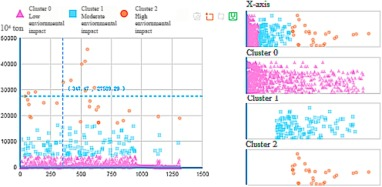
\includegraphics[width=0.8\textwidth]{figures/liu_assessmentOfIndustries/liu_environmentalPerformance.jpg}
    \caption{Multi-Industries Clustering Result based on the $SO_2$ Emission \cite{LIU-BDE}}
    \label{fig:multi_industries_clustering_result_environemental_performance}
\end{figure}

\begin{table}[h]
    \centering
    \begin{tabular}{c|c|c|c|c}
        \textbf{Fields} & \textbf{Sum} & \textbf{Cluster 0} & \textbf{Cluster 1} & \textbf{Cluster 2} \\
        \hline
        Chemical Industry & 144 & 138 & 0 & 6 \\
        Coal Mining and Washing Industry & 60 & 54 & 4 & 2 \\
        Black Metal Smelting & 75 & 53 & 6 & 16 \\
        Textile Industry & 49 & 49 & 0 & 0 \\
        Paper Products Industry & 47 & 42 & 0 & 5 \\
        Electricity, Heat Industry & 384 & 274 & 18 & 92 \\
    \end{tabular}
    \caption{Snippet of the Multi-Industries Clustering Results based on the $SO_2$ Emission \cite{LIU-BDE}}
    \label{tab:multi_industries_clustering_results_based_on_the_so2_emission}
\end{table}

% \paragraph*{MAL-HBP:}
% % Wie soll dieser Paragraph strukturiert sein?
% % 1. Allgemeine Ergebnisse ansprechen
% % 2. Auf ein Beispiel eingehen (in diesem Fall das Clustering und die Tabelle)
% The research is conducted on the total data set and the data split into the disctinct households.
% Also, the data is split into winter and summer data.

% After clustering the whole dataset several assumptions are made.
% First, dominant routines are spotted by averaging the total dataset.
% This leads to a dual peak average as shown in \autoref{fig:total_data_averaging}.
% Therefore, practices can be socially shared.
% Also, different consumption practices for the summer and winter seasons are found.

% After applying k-means to each household, routinized households and less routinized households can be identified.
% Routinized households (\autoref{fig:routinized_household}) show a smaller number of clusters and therefore less HSOPs than less routinized households (\autoref{fig:non_routinized_household}).
% Due to the application of social theories and the survey, two assumptions can be made:
% \begin{itemize}
%     \item Variable lifestyles with different work commitments (e.g. working from home) or family structures (e.g. having children) alter the energy consumption of households \cite{KUR-HBP}.
%     \item If occupants are routinized, their behaviors are repetitive \cite{BRE-EWP}.
% \end{itemize}

\begin{figure}
    \centering
    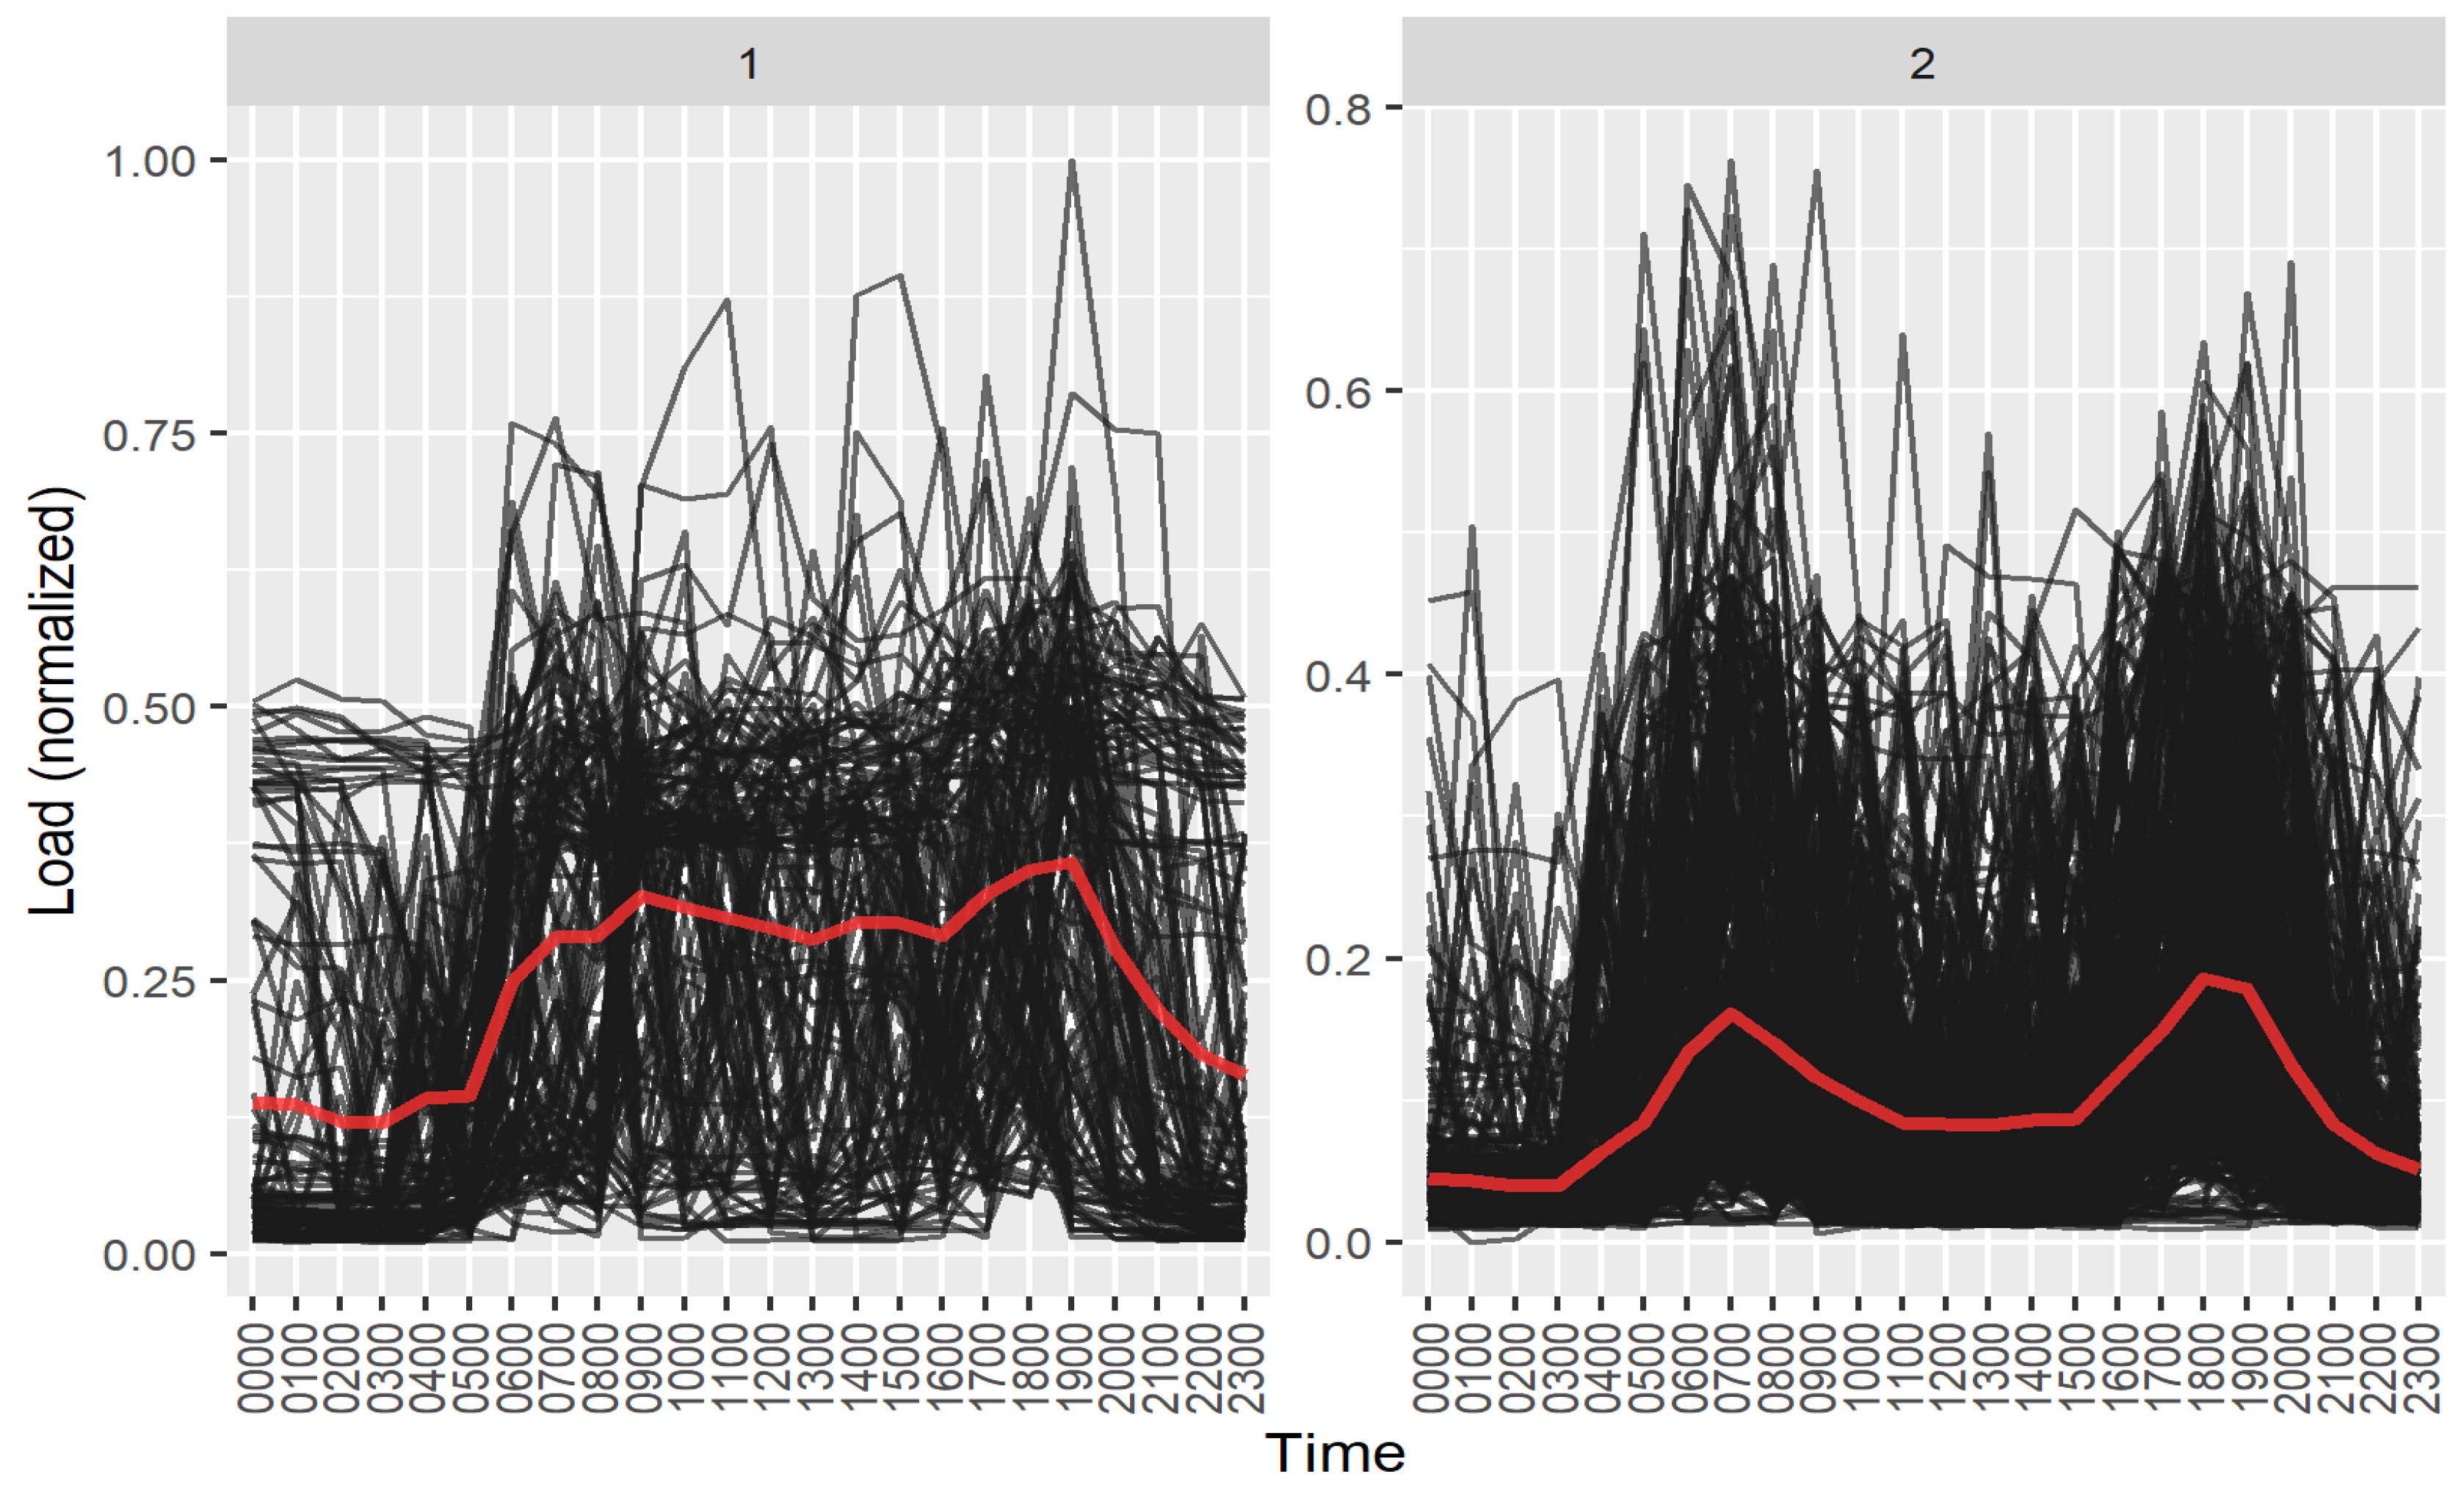
\includegraphics[width=0.5\textwidth]{figures/malatesta_hsop/malatesta_routinisedHousehold.jpg}
    \caption{K-Means resulting in a Routinised Household Using all Year Energy Data \cite{MAL-HBP}}
    \label{fig:routinized_household}
\end{figure}

\begin{figure}
    \centering
    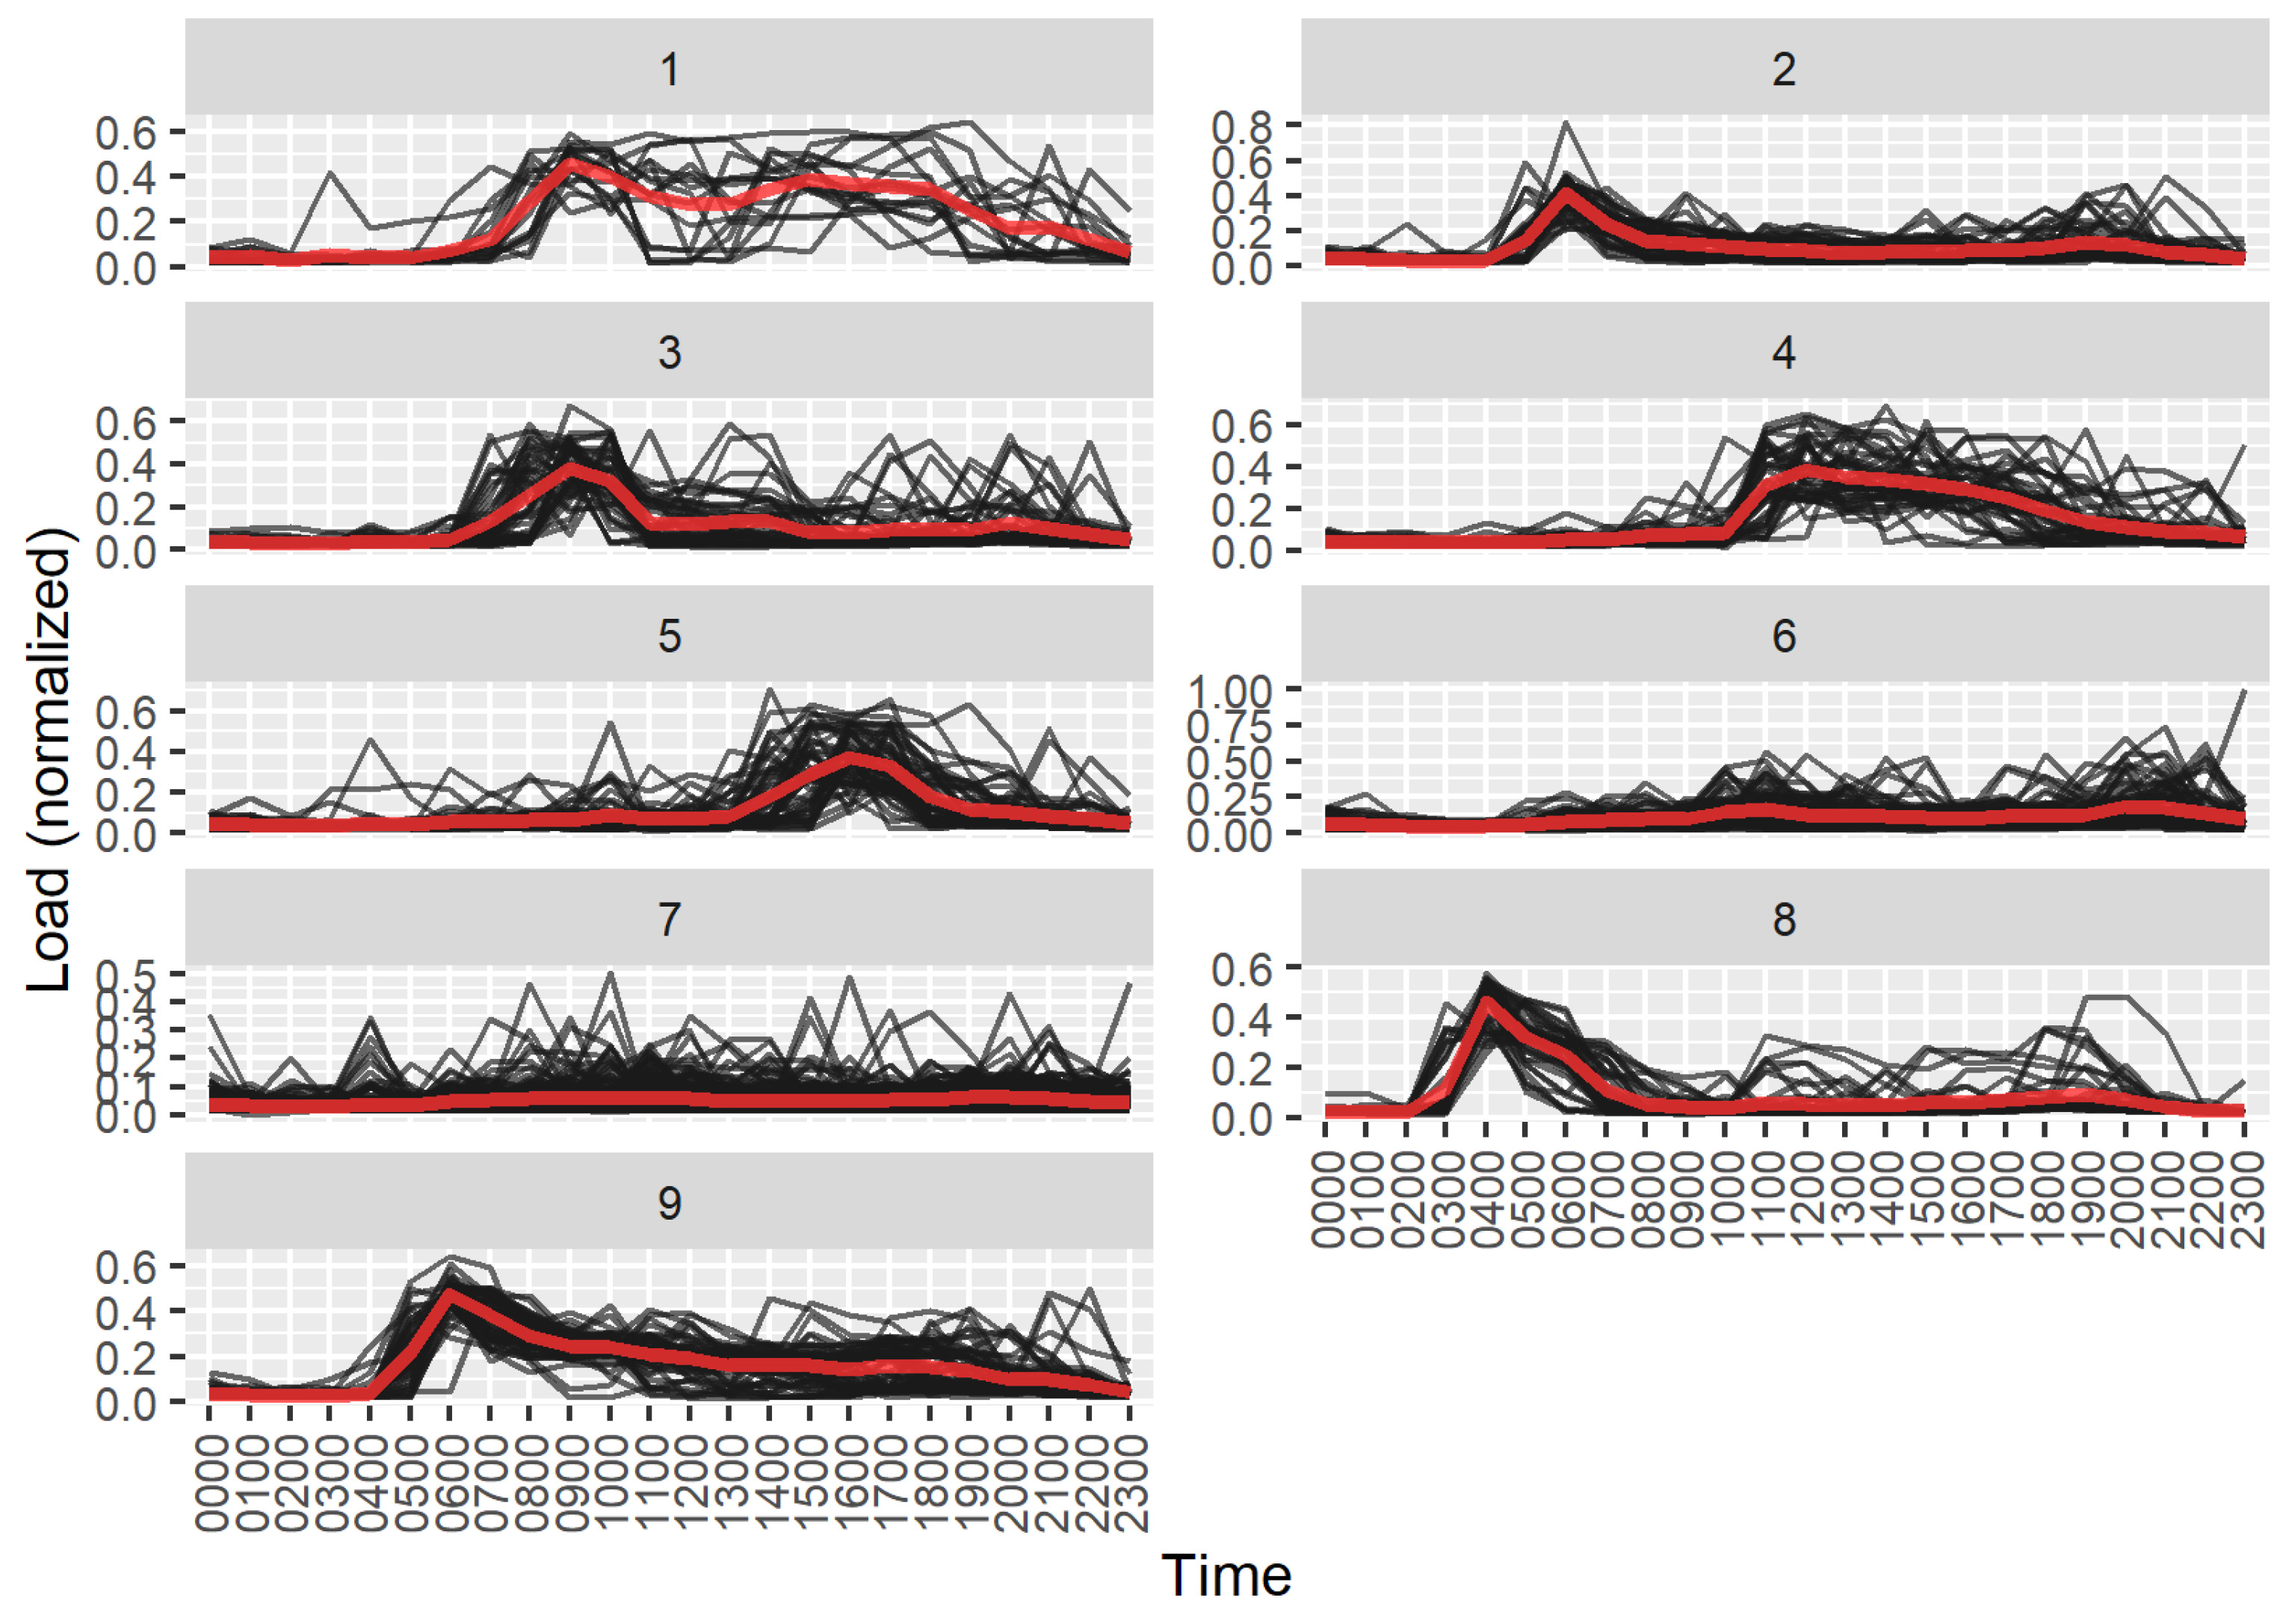
\includegraphics[width=0.5\textwidth]{figures/malatesta_hsop/malatesta_unroutinisedHousehold.jpg}
    \caption{K-Means resulting in an Unroutinised Household Using all Year Energy Data \cite{MAL-HBP}}
    \label{fig:non_routinized_household}
\end{figure}

\begin{figure}
    \centering
    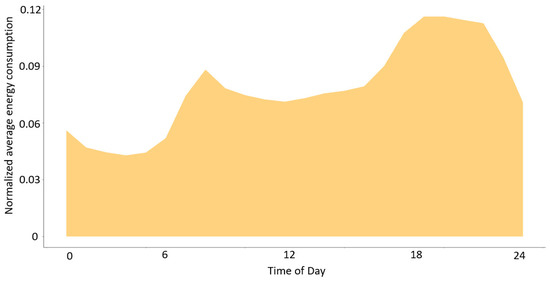
\includegraphics[width=0.5\textwidth]{figures/malatesta_hsop/malatesta_totalDataAveraging.jpg}
    \caption{Total Data Averaging \cite{MAL-HBP}}
    \label{fig:total_data_averaging}
\end{figure}

% \paragraph*{What do both Summaries have in Common?}
% \begin{itemize}
%     \item Identifying and comparing of:
%     \begin{itemize}
%         % \item Patterns (Malatesta => Habits patterns, clustering of the whole profile; Liu => Some industry sectors are in general more energy consuming than others)
%         % \item Tendencies (Liu => Some industry sectors being represented in cluster 0 and cluster 2)
%         % \item (Best Practices) topic for the conclusion
%         % \item Outliers (Malatesta => Routinised and less routinized households)
%         % \item Shared and individual practices/habits (Malatesta => Whole data clustering)
%         % \item Thresholds (Liu => Limits in consumption/emissions are spotted)
%         \item Characteristics of each cluster (Both => Clusters represent a certain characteristic (Practice/Certain Metric); Malatesta => Some practices can be tracked to a certain practice)
%         \item Dominant characteristics/practices (Malatesta => Some habits reappeared several times in multiple clusterings)
%         % \item Key industries for energy saving incentives (Liu => Some industry sectors are in general more energy consuming than others)
%     \end{itemize}
% \end{itemize}



\paragraph*{Industry:}
% Grundlegende Idee: Ergebnisse in Industrie und Private Housing unterteilen, general findings werden separat für alle Paper gezeigt
% Dabei die jeweiligen Findings am Beispiel zeigen
% Alles was eigentlich aus dem Background klar sein sollte wird dorthin geschoben
% => Nur auf die Ergebnisse aus dem Paper eingehen, dabei nicht werten oder eigene Schlussfolgerungen ziehen
% Die Schritte, wie man zu den Ergebnissen kommt, sollen aus dem Background bereits klar sein
Applying k-means with a fixed value of $k=3$, the datasets are separated into low-, mid-, and highly-efficient industry sectors or companies within these sectors.
Therefore, general patterns are detected and compared.
Spotting these general characteristics' thresholds and characteristic metrics are determined.
A clustering example of the environmental impact measured on $SO_2$ emissions is shown in \autoref{fig:multi_industries_clustering_result_environemental_performance}.
General high-consuming, low-efficient industry sectors are spotted, in this case for example the black metal smelting industry as shown in \autoref{tab:multi_industries_clustering_results_based_on_the_so2_emission}.
Most clusters are represented in one cluster yet some are scattered over several clusters.
\autoref{tab:multi_industries_clustering_results_based_on_the_so2_emission} shows the electric power and heat supply industry as a fitting example.
Mostly this is due to a few companies of the reviewed industry sector being less efficient.
This helps in identifying outliers, which means less efficient sectors and companies.
Therefore, applying k-means to the given dataset helps in finding a starting point in industry sectors and distinct companies for putting energy-saving incentives into action.

\paragraph*{Private Housing:}
Again, patterns are detected using k-means, yet in a different context with different interpretations.
Averaging the whole dataset (\autoref{fig:total_data_averaging}) provided insights into dominant practices and habits that are socially shared among the residents of the precinct.
Also, HSOPs are different for the summer and winter seasons.
These assumptions can be made due to k-means laying the groundwork for applying social theory and the survey results after the clustering process.
The \texttt{dual peak model} with dip midday is the average consumption habit of the monitored precinct.
Analyzing the clustering on the whole dataset gave insights into how habits are shared between different households.
Dominant HSOPs are identified with general characteristics being found.
Clustering single household data gave insights into how flexibility and routine affect different energy consumption practices.
The results varied between two (\autoref{fig:routinized_household}) up to nine (\autoref{fig:non_routinized_household}) clusters per household.
Due to the application of social theories and surveying the residents, two assumptions are made:
\begin{itemize}
    \item Variable lifestyles with different work commitments (e.g. working from home) or family structures (e.g. having children) alter the energy consumption of households \cite{KUR-HBP}.
    \item If occupants are routinized, their behaviors are repetitive \cite{BRE-EWP}.
\end{itemize}
Therefore, applying k-means to this data reveals the hidden knowledge of HSOPs and identifies starting points for developing best practices in energy consumption.

\section{Identifying and Differentiating Natural Disaster- and Electrical Fault-Impacted Load Profiles}
\label{sec:identifying_and_differentiating_natural_disaster_and_electrical_fault_impacted_load_profiles}